\chapter{PandaXIII项目介绍}
\label{chapter:intro}
%\pkuthssffaq % 中文测试文字。

正如上文所说的,无中微子双Beta衰变事件是一种极其稀有的事件,既有实验已经给去它的半衰期$T^{0\nu}_1/2>1.07\times10^{26}$年,需要达成给出中微子质量顺序这一中期目标至少需要1吨量级的衰变元素。因而相应的实验难点便是以下四点:
\begin{enumerate}
    \item 顺利制造生产出吨级的可能发生NLDBD事件的放射性元素。
    \item 探测器具有极佳的能量分辨率和位置分辨率,能够准确的捕捉到NLDBD事件。
    \item 探测器本底噪声很低,在灵敏区域的背景事件应该小于0.1个每吨每年。
    \item 合适的数据处理方法来区分NLDBD事件以及和背景事件
\end{enumerate}
在PandaXIII实验中我们通过适当的选择衰变元素以及合理设计构造探测器结构等诸多方法来解决上述四点难点,以此保障能够顺利的达成探测NLDBD事件的实验目标。

\section{元素选择}

在诸多可以发生 NLDBD 事件的放射性元素中,PandaXIII选取了$^{136}$Xe作为目标,因为其在自然界中含量较为丰富,因而相对便宜。再有$^{136}$Xe作为衰变元素的同时也可以作为探测器的敏感气体,因而使用它可以制造出相当巨大的气体探测器。该元素 NLDBD 事件释放出的总能量为$Q_{\beta\beta}=2458keV$,这个能量相对较高,能够避免低能的背景辐射,但是在$Q_{\beta\beta}$附近也有来自$^{214}$Bi和$^{208}$Tl两种元素 Gamma 衰变的本底噪声,其中$^{214}$Bi会产生2448keV的$\gamma$射线,只比$Q_{\beta\beta}$低了10keV。这两种元素作为$^{238}$U和
$^{232}$Th衰变链中的中间元素广泛存在于自然界的各个角落中,因而对PandaXIII实验提出了巨大的挑战。

PandaXIII使用了10bar的高压气氙作为探测气体,其中$^{136}$Xe的丰度为90\%。同时为了配合电子学读出系统,气体混合了1\%的TMA(trimethylamine)来增强信号质量,根据NEXT实验的相关研究,使用该混合气体作为探测介质能够达到3\%的能量分辨率\supercite{azevedoh2015accurate}。

\section{探测器构造}

为了能够达到优秀的能量分辨率,PandaxIII实验计划建造5个200kg级别的高压气氙时间漂移室(time projection chamber, TPC)作为 NLDBD 的探测器,如图\ref{fig:detector}左所示。高压气体时间漂移室的技术在上个世纪90年代便已经成熟,相对与液体漂移时而言它能够提供更为优良的能量分辨率,如果使用直接读出电离电子数目的读取器件,高压气体TPC的分辨率能够接近达到液体的10倍。高压气体时间漂移室另外一个十分巨大的优势是能够较好的保留 NLDBD 事件的径迹,配合像素或者条状读出事件的径迹可以十分便捷的重建出,利用径迹信息可以极高效率的分辨出本地事件和 NLDBD 事件,从而能够几十倍的压低背景噪声。本文第\ref{chapter:cnn}章着重介绍了使用CNN分辨事件压低本地的方法。

\begin{figure}[tbp]
    \centering
    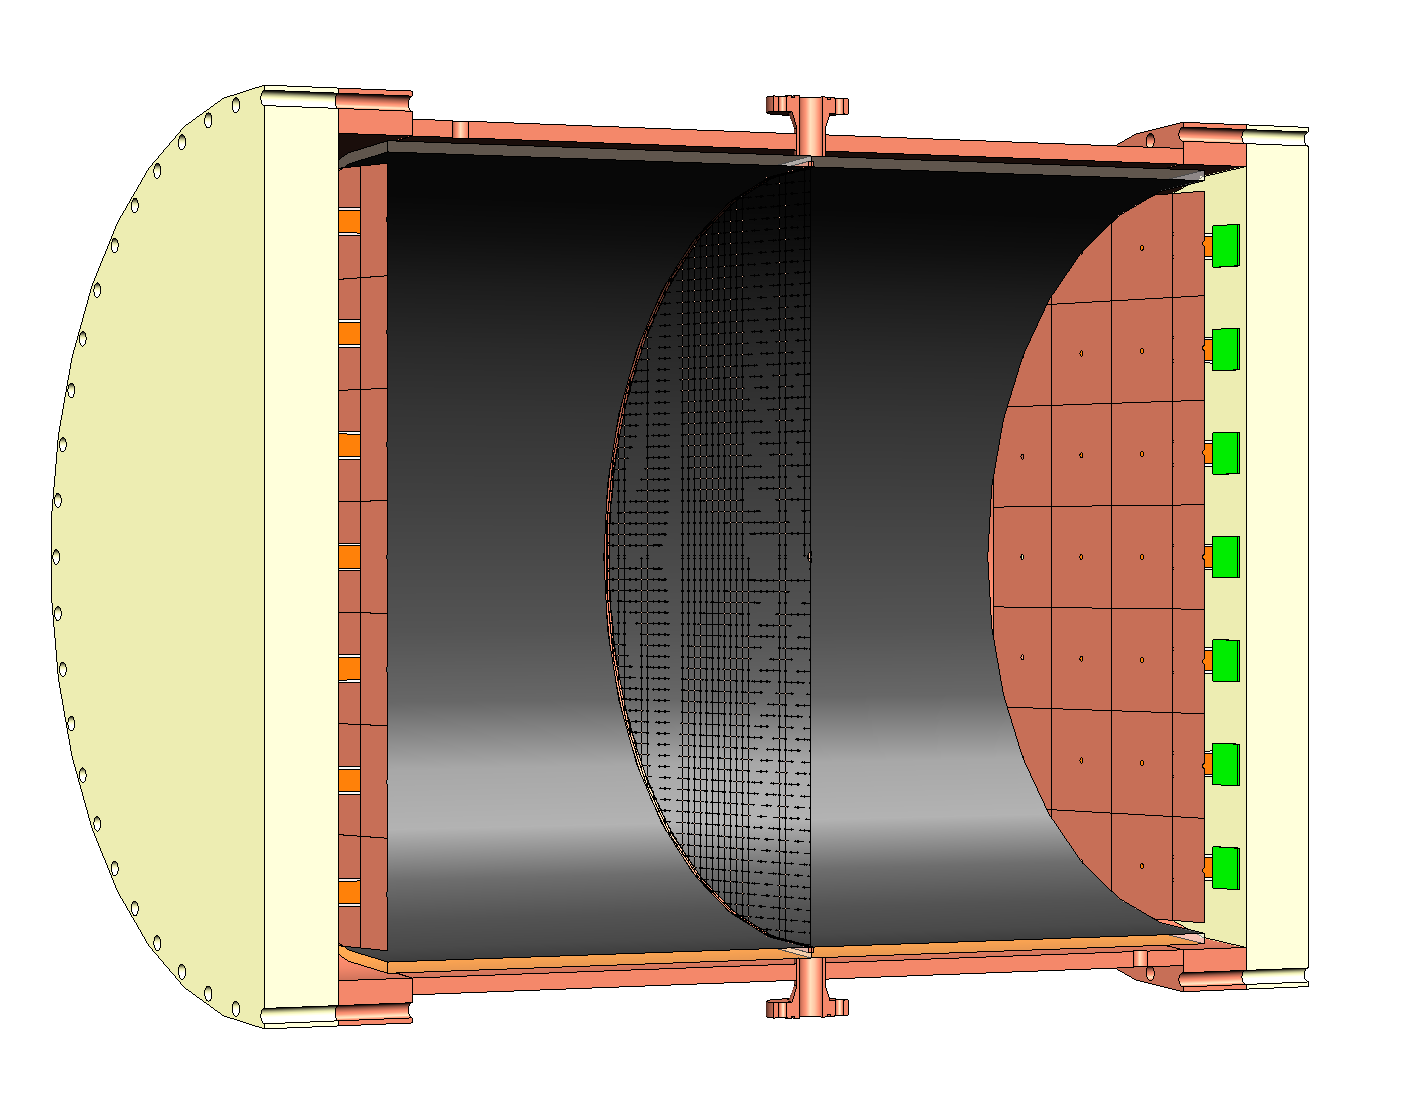
\includegraphics[width=0.4\columnwidth]{pic/fig1.png}
    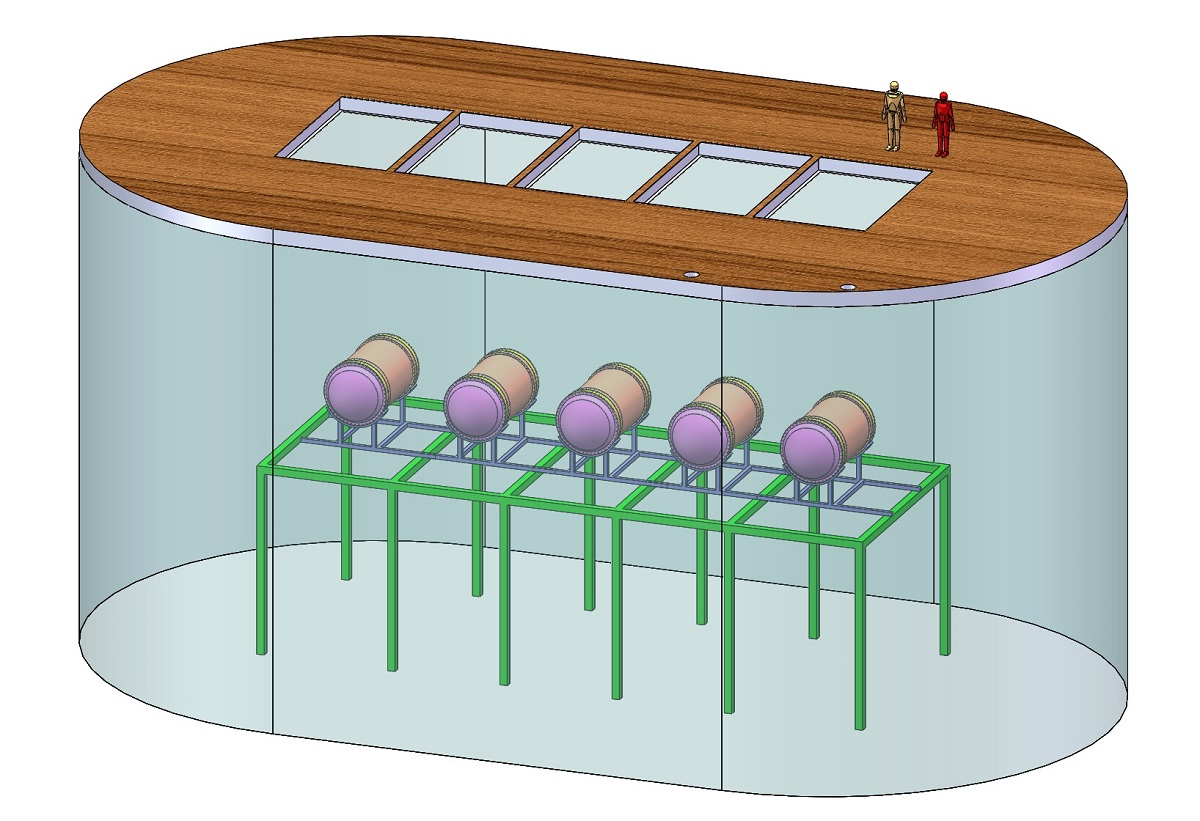
\includegraphics[width=0.4\columnwidth]{pic/fig2.jpg}
    \caption{左图:PandaXIII时间漂移室结构示意图。右图:5个TPC被放置在屏蔽水池示意图。\supercite{cdr}}
    \label{fig:detector}
\end{figure}
    
探测器主体是一个内高2米,内径1.5米的柱形压力铜罐,使用了高纯度无氧铜制作,总容积约3.5m$^3$。在铜罐中心部分有圆形网状极板,在铜罐内壁有99个圆形铜环,铜环之间以及铜环与内壁之间使用聚四氟乙烯(PTFE)做隔离和支撑,铜环,极板之间形成场笼,提供延罐体轴心方向,强度为1kV/cm的漂移电场。铜罐壁自身厚度约30
mm,两端厚度约150mm,整体放置于在如图\ref{fig:detector}右侧一个尺寸为27x15x13米的水池中,利用超纯水来屏蔽来自周围环境的本底射线。同时整体实验位于中国锦屏地下实验室中,利用隧道上方2500米厚的山岩屏蔽宇宙射线。对于探测器自身材料产生的本底射线,PandaXIII实验通过适当的材料选择和探测器构造来降低这部分背景干扰,根据近年的一些研究,一些商业无氧铜中铀和钍的含量可以低于0.1个ppt(part per trillion)\supercite{abgrall2016majorana},是不锈钢材质的千分之一以上。本文第\ref{chapter:background}章主要介绍了使用Geant4模拟并分析探测器材料所带来的具体影响。

\section{电子学读出}

为了提高探测器的分辨率,PandaXIII实验使用了新型的被称作Micromegas的读出系统。该读出通过直接收集电离后的漂移电子来获取信号,结构相对简单分辨率高,也更容易控制由自身材料带来本地污染。根据现有的对于 Microbulk Micromeags(MM,一种部分实现的Micromegas)读出系统做了详细的研究,在目标$Q_{\beta\beta}$附近它配合10Bar
气氙和TMA混合气体组成的高压探测器能够达到3\%的能量分辨率。PandaXIII实验前期会直接向 CERN(European Organization for Nuclear Research,欧洲核子研究中心)订购Microbulk Micromegas成品,在项目的中后期将会试图对读出系统做进一步的改进以达到1\%的能量分辨率。

在读出系统的电子学部分中电路可能会泄露的部分电子,电子电气元器件也相对不干净,可能带来较大的背景污染,对实验造成一定的影响,因而在探测器设计中将读出系统的电子学部分放置在了铜罐的两端,通过150mm厚度的铜体来屏蔽这一部背景噪声。同时为了能够重建得到被探测事件的径迹,读出系统需要是一个像素读出,这样的话大量的通道数目对于电子学的设计也是一个挑战。关于电子学以及数据获取系统的具体设计参见中期设计报告\supercite{cdr}

\section{PandaXIII实验设计总结及模拟工作}

为了探测寻找到NLDBD这样一种及其稀有的事件,PandaXIII实验在各个方面上都做了相当细致的考虑和设计,总结如下:
\begin{itemize}
    \item 提高探测器的灵敏度。
    \begin{itemize}
        \item 使用10bar高压气Xe+TMA时间漂移室作为探测器。
        \item 使用新型的Microbulk MicroMegas读出系统直接捕获漂移电子。
    \end{itemize}
    \item 减少背景干扰。
    \begin{itemize}
        \item 设计和建造探测器时控制探测器材料的本地辐射水平。
        \item 将探测器放置与中国锦屏地下实验室中的高纯水水池中,以此屏蔽宇宙射线以及环境中的本地辐射。
        \item 通过合理的探测器结构设计减少一些由材料带来的本地辐射。
    \end{itemize}
    \item 寻找合适的算法高效的分辨背景事件和NLDBD时间,进而极大的提高探测器的探测效率。
\end{itemize}
在这些考虑和设计的过程中,模拟工作相当的重要,为整个实验提供了前期的数据支持。通过模拟我们可以得到不同设计的探测器灵敏度,可以得到使用不同材料时本地噪声的量级,并可以通过这些数据来指导设计细节的改进和材料的具体挑选。除此之外,模拟工作也能帮助读出系统以及探测器电子学参数的优化,以及探测器的标定设计。在PandaXIII实验前期建造原型探测器以检验设计的可行性时,模拟工作也能够为验证实验结果,解释未知问题提供巨大的帮助。最为重要的是,PandaXIII实验十分需要一种优异良好的本地事件和信号事件的区分鉴别方法,而鉴别方法的数据来源则需要由模拟工作提供。综合而言模拟工作对PandaXIII实验相当的重要,本文后续的几章中详细介绍了模拟工作的细节。

% vim:ts=4:sw=4
